\documentclass[12pt]{article}

\usepackage[margin=0.7in,letterpaper]{geometry}
\usepackage{enumitem}
\usepackage{graphicx}
\usepackage{tikz}%,graphicx,wrapfig}
\usepackage{mathpazo}
\usepackage[scaled]{helvet}
\usepackage{siunitx}

\usetikzlibrary{decorations.pathmorphing,patterns}

\sisetup{number-math-rm=\mathnormal}

\renewcommand{\familydefault}{\sfdefault}

\newcommand{\pic}[2]{\includegraphics[width=#1\textwidth]{#2}}
\newcommand{\magdir}[2]{$#1\;[\mathrm{#2}]$}
\newcommand{\mb}[1]{\mathbf{#1}}

\begin{document}

\begin{center}
  Student \#: \underline{\hspace{1in}}\hspace{1.9in}
  Student Name: \underline{\hspace{2in}}\\
  \vspace{0.3in}
  {\LARGE
    AP Physics \hspace{0.68in} Class 7: Simple Harmonic Motion
  }
\end{center}

\begin{enumerate}[leftmargin=50pt,label=\underline{\hspace{0.4in}} \arabic*.]

\item A simple pendulum has a mass $m$, length $L$, and period $T$. If the
  pendulum mass is replaced by a mass of $2m$, the period will be
  \begin{enumerate}[noitemsep,topsep=0pt]
  \item doubled
  \item halved
  \item quartered
  \item quadrupled
  \item unchanged
  \end{enumerate}

\item A mass oscillates on the end of a spring that obeys Hooke’s law. Which of
  the following statements is true?
  \begin{enumerate}[noitemsep,topsep=0pt]
  \item The amplitude of oscillation is equal to the potential energy of the
    spring.
  \item The kinetic energy of the oscillating mass is constant.
  \item The maximum potential energy occurs when the mass reaches the
    equilibrium position.
  \item The potential energy of the spring at the amplitude is equal to the
    kinetic energy at the equilibrium position.
  \item The kinetic energy of the spring at the amplitude is equal to the
    potential energy at the equilibrium position.
  \end{enumerate}

\item A superball is dropped from a height of \SI{5.0}{meters} above a floor.
  The ball bounces off the floor in a perfectly elastic collision so that it
  rises to the same height with each bounce. The motion of the ball can be
  described as
  \begin{enumerate}[noitemsep,topsep=0pt]
  \item harmonic motion with a period of $2$ \si{s}
  \item harmonic motion with a period of $1$ \si{s}
  \item harmonic motion with a period of $1⁄2$ \si{s}
  \item motion with a constant velocity
  \item motion with a constant momentum
  \end{enumerate}

\item An object oscillates in simple harmonic motion along the $x$-axis
  according to the equation $x = 6 \cos(4t)$. The period of oscillation of the
  object is
  \begin{enumerate}[noitemsep,topsep=0pt]
  \item $1⁄4$ \si{s}
  \item\SI{4}{s}
  \item\SI{\pi/4}{s}
  \item\SI{\pi/2}{s}
  \item\SI{4\pi}{s}
  \end{enumerate}    

\item A mass $m$ oscillates on the end of a string of length $L$. The frequency
  of the pendulum is $f$. How would you increase the frequency of the
  pendulum to $2f$?
  \begin{enumerate}[noitemsep,topsep=0pt]
    \item Increase the length of the pendulum to $4L$
    \item Decrease the length of the pendulum to $1⁄4L$
    \item Increase the length of the pendulum to $2L$
    \item Decrease the length of the pendulum to $1⁄2L$
    \item Decrease the mass of the pendulum to $1⁄2m$
  \end{enumerate}

  \begin{center}
    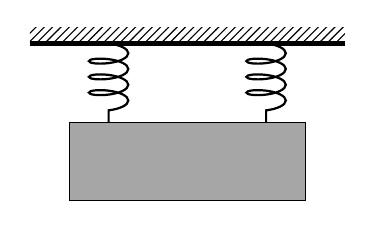
\begin{tikzpicture}
      \fill [pattern=north east lines] (-2,4) rectangle (2,4.2);
      \draw[ultra thick] (-2,4)--(2,4);
      \draw[thick,
        decoration={aspect=0.3,segment length=2mm, amplitude=2.5mm, coil},
        decorate] (-1,4)--(-1,3);
      \draw[thick,
        decoration={aspect=0.3,segment length=2mm, amplitude=2.5mm, coil},
        decorate] (1,4)--(1,3);
      \draw[fill=gray!70](-1.5,3) rectangle(1.5,2);
    \end{tikzpicture}
  \end{center}

\item A mass hangs from two parallel springs, each with the same spring
  constant $k$. Compared to the period $T$ of the same mass oscillating on
  one of the springs, the period of oscillation of the mass with both
  springs connected to it is
  \begin{enumerate}[noitemsep,topsep=0pt]
  \item $\frac{1}{4}T$
  \item $\frac{1}{2}T$
  \item $T$ (unchanged)
  \item $2T$
  \item $4T$
  \end{enumerate}

\item Which of the following is generally true for an object in simple
  harmonic motion on a spring of constant k?
  \begin{enumerate}[noitemsep,topsep=0pt]
  \item The greater the spring constant $k$, the greater the amplitude of the
    motion.
  \item The greater the spring constant $k$, the greater the period of the
    motion.
  \item The greater the spring constant $k$, the greater the frequency of the
    motion.
  \item The lower the spring constant $k$, the greater the frequency of the
    motion.
  \item The lower the spring constant $k$, the greater the kinetic energy of
    the motion.
  \end{enumerate}
\end{enumerate}

\noindent Questions 8-10: A harmonic oscillator follows the equation
$\displaystyle \frac{d^2x}{dt^2}=-4x$. The spring constant $k$ is \SI{4}{N/m}.

\begin{enumerate}[leftmargin=50pt,label=\underline{\hspace{0.4in}} \arabic*.]
  \setcounter{enumi}{7}
\item The angular frequency ω of the harmonic motion is
  \begin{enumerate}[noitemsep,topsep=0pt]
  \item zero
  \item\SI{2}{rad/s}
  \item\SI{4}{rad/s}
  \item\SI{8}{rad/s}
  \item\SI{16}{rad/s}
  \end{enumerate}
  
\item The mass $m$ oscillating on the spring is
  \begin{enumerate}[noitemsep,topsep=0pt]
  \item\SI{1}{\kg}
  \item\SI{2}{\kg}
  \item\SI{4}{\kg}
  \item\SI{8}{\kg}
  \item\SI{16}{\kg}
  \end{enumerate}
  
\item The period $T$ of oscillation is
  \begin{enumerate}[noitemsep,topsep=0pt]
  \item zero
  \item $\pi/4$\si{s}
  \item $\pi/2$\si{s}
  \item $\pi$  \si{s}
  \item $2\pi$ \si{s}
  \end{enumerate}

\item A pendulum of length $L$ has a period of \SI{2}{\s} on Earth. A planetary
  explorer takes the same pendulum of length $L$ to another planet where
  its period is \SI{1}{\s}. The gravitational acceleration on the surface of
  this planet is most nearly
  \begin{enumerate}[noitemsep,topsep=0pt]
  \item $8 g$
  \item $4 g$
  \item $2 g$
  \item $1⁄2 g$
  \item $1⁄4 g$
  \end{enumerate}

  \begin{center}
    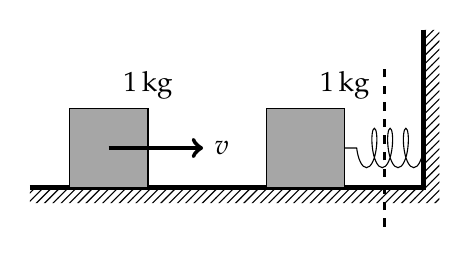
\begin{tikzpicture}
      \fill [pattern=north east lines] (-5,0)--(0,0)--(0,2)--(0.2,2)--(0.2,-0.2)
      --(-5,-0.2)--cycle;
      \draw[ultra thick] (-5,0)--(0,0)--(0,2);
      \draw[decoration={aspect=0.3,segment length=2mm, amplitude=2.5mm, coil},
        decorate] (0,0.5)--(-1,0.5);
      \draw[fill=gray!70](-2,0) rectangle(-1,1) node[above]{\SI{1}{\kg}};
      \draw[fill=gray!70](-4.5,0) rectangle(-3.5,1) node[above]{\SI{1}{\kg}};
      \draw[ultra thick,->](-4,0.5)--(-2.8,0.5) node[pos=1,right]{$v$};
      \draw[very thick,dashed](-0.5,-0.5)--(-0.5,1.5);
    \end{tikzpicture}
  \end{center}
  
\item\vspace{-0.2in} A block of mass \SI{1.0}{\kg} is sliding on a frictionless horizontal
  surface with a speed of \SI{4.0}{m/s} when it collides inelastically with
  another \SI{1.0}{kg} block attached to a spring. The spring compresses a
  distance of \SI{0.5}{m} after the collision. The force constant $k$ of the
  spring is
  \begin{enumerate}[noitemsep,topsep=0pt]
  \item\SI{2}{N/m}
  \item\SI{4}{N/m}
  \item\SI{8}{N/m}
  \item\SI{16}{N/m}
  \item\SI{32}{N/m}
  \end{enumerate}

  \begin{center}
    \pic{0.5}{projectile.png}
  \end{center}
  
\item A block of mass \SI{0.5}{kg} rests up against a compressed spring of force
  constant \SI{5}{N/m}. The spring is released, and the block travels a distance
  of \SI{1.0}{m} when the block leaves the spring at the edge of the horizontal
  frictionless table, and is projected to the floor. The table is \SI{1.5}{m}
  high. The horizontal distance from the table the block lands on the floor is
  \begin{enumerate}[noitemsep,topsep=0pt]
  \item\SI{1.2}{\metre}
  \item\SI{1.7}{\metre}
  \item\SI{2.1}{\metre}
  \item\SI{2.8}{\metre}
  \item\SI{3.4}{\metre}
  \end{enumerate}
\end{enumerate}


\noindent The following questions are ``review'' questions for kinematics.

\begin{enumerate}[leftmargin=50pt,label=\underline{\hspace{0.4in}} \arabic*.]
  \setcounter{enumi}{13}

\item  A golf ball is hit from level ground and has a horizontal range of
  \SI{100}{m}. The ball leaves the golf club at an angle of \ang{60} to the
  level ground. At what other angle(s) can the ball be struck at the same
  initial velocity and still have a range of \SI{100}{m}?
  \begin{enumerate}[noitemsep,topsep=0pt]
  \item\ang{30}
  \item\ang{20} and \ang{80}
  \item\ang{10} and \ang{120}
  \item\ang{45} and \ang{135}
  \item There is no other angle other than \ang{60} in which the ball will have
    a range of \SI{100}{m}.
  \end{enumerate}
  \begin{center}
    \pic{0.3}{golf.png}
  \end{center}


%\item Two disks are fixed to a vertical axle that is rotating with a constant
%  angular speed $\omega$. The smaller disk has a mass $m$ and a radius $r$, and
%  the larger disk has a mass $2m$ and radius $2r$. The general equation for the
%  rotational inertia of a disk of mass $M$ and radius $R$ is $\frac{1}{2}MR^2$.
%  The ratio of the angular momentum of the larger disk to the smaller disk is\\
%  \begin{minipage}{0.3\textwidth}
%    \begin{enumerate}[noitemsep,topsep=0pt]
%    \item$1/4$
%    \item$4/1$
%    \item$1/2$
%    \item$2/1$
%    \item$8/1$
%    \end{enumerate}
%  \end{minipage}
%  \begin{minipage}{0.6\textwidth}
%    \pic{.5}{2disks.png}
%  \end{minipage}
%  
%\item A light rod has a mass attached at each end. At one end is a \SI{6}{\kg}
%  mass, and at the other end is a \SI{3}{\kg} mass. An axis can be placed at
%  any of the points shown. Through which point should an axis be placed so that
%  the rotational inertia is the greatest about that axis?
%  
%  \begin{minipage}{0.3\textwidth}
%    \begin{enumerate}[noitemsep,topsep=0pt]
%    \item A
%    \item B
%    \item C
%    \item D
%    \item E
%    \end{enumerate}
%  \end{minipage}
%  \begin{minipage}{0.6\textwidth}
%    \pic{.8}{light-rod.png}
%  \end{minipage}
%
%\item Two wheels are attached to each other and fixed so that they can only
%  turn together. The smaller wheel has a radius of $r$ and the larger wheel
%  has a radius of $3r$. The two wheels can rotate together on a frictionless
%  axle. Three forces act tangentially on the edge of the wheels as shown.
%  The magnitude of the net torque acting on the system of wheels is\\
%  \begin{minipage}{0.3\textwidth}
%    \begin{enumerate}[noitemsep,topsep=0pt]
%    \item$Fr$
%    \item$2Fr$
%    \item$3Fr$
%    \item$4Fr$
%    \item$6Fr$
%    \end{enumerate}
%  \end{minipage}
%  \begin{minipage}{0.6\textwidth}
%    \pic{.5}{2wheels.png}
%  \end{minipage}
%  \newpage
%
%\item Astronauts are conducting an experiment in a negligible gravity
%  environment. Two spheres of mass m are attached to either end of a
%  light rod. As the rod and spheres float motionless in space, an astronaut
%  launches a piece of sticky clay, also of mass m, toward one of the
%  spheres so that the clay strikes and sticks to the sphere perpendicular to
%  the rod. Which of the following statements is true of the motion of the
%  rod, clay, and spheres after the collision?
%  
%  \begin{minipage}{0.6\textwidth}
%    \begin{enumerate}[topsep=5pt]
%    \item Linear momentum is not conserved, but angular momentum is conserved.
%    \item Angular momentum is not conserved, but linear momentum is conserved.
%    \item Kinetic energy is conserved, but angular momentum is not conserved.
%    \item Kinetic energy is conserved, but linear momentum is not conserved.
%    \item Both linear momentum and angular momentum are conserved, but kinetic
%      energy is not conserved.
%    \end{enumerate}
%  \end{minipage}
%  \begin{minipage}{0.3\textwidth}
%    \pic{1}{collision1.png}
%  \end{minipage}
%  
%\item One end of a stick of length $L$, rotational inertia $I$, and mass $m$ is
%  pivoted on an axle with negligible friction at point $P$. The other end is
%  tied to a string and held in a horizontal position. When the string is cut,
%  the stick rotates counterclockwise. The angular speed $\omega$ of the stick
%  when it reaches the bottom of its swing is\\
%  \begin{minipage}{0.3\textwidth}
%    \begin{enumerate}[noitemsep,topsep=0pt]
%    \item$\displaystyle\frac{mgL}{I}$
%    \item$\displaystyle\sqrt{\frac{mgL}{I}}$
%    \item$\displaystyle\sqrt{\frac{2mgL}{I}}$
%    \item$\displaystyle\sqrt{\frac{mgL}{2I}}$
%    \item$\displaystyle\sqrt{\frac{4mgL}{I}}$
%    \end{enumerate}
%  \end{minipage}
%  \begin{minipage}{0.65\textwidth}
%    \pic{.7}{end-of-stick.png}
%  \end{minipage}
%
%\item A belt is wrapped around two wheels as shown. The smaller wheel has
%  a radius $r$, and the larger wheel has a radius $2r$. When the wheels turn,
%  the belt does not slip on the wheels, and gives the smaller wheel an
%  angular speed $\omega$. The angular speed of the larger wheel is
%  
%  \begin{minipage}{0.3\textwidth}
%    \begin{enumerate}[noitemsep,topsep=0pt]
%    \item $\displaystyle \omega$
%    \item $\displaystyle 2\omega$
%    \item $\displaystyle \frac{1}{2}\omega$
%    \item $\displaystyle \frac{1}{4}\omega$
%    \item $\displaystyle 4\omega$
%    \end{enumerate}
%  \end{minipage}
%  \begin{minipage}{0.65\textwidth}
%    \pic{.7}{wheels.png}
%  \end{minipage}  
%  \newpage
%
%\item A disk is mounted on a fixed axle. The rotational inertia of the disk is
%  $I$. The angular velocity of the disk is decreased from $\omega_0$ to
%  $\omega_f$ during a time $\Delta t$ due to friction in the axle. The
%  magnitude of the average net torque acting on the wheel is
%  \begin{enumerate}[noitemsep,topsep=0pt]
%  \item $\displaystyle\frac{\omega_f-\omega_0}{\Delta t}$
%  \item $\displaystyle\frac{(\omega_f-\omega_o)^2}{\Delta t}$
%  \item $\displaystyle\frac{I(\omega_f-\omega_o)}{\Delta t}$
%  \item $\displaystyle\frac{I(\omega_f-\omega_o)^2}{\Delta t}$
%  \item $\displaystyle\frac{I(\omega_f-\omega_o)}{\Delta t^2}$
%  \end{enumerate}
%
%\item The average power developed by the friction in the axle of the disk
%  from the previous question to bring it to a complete stop is
%  \begin{enumerate}[noitemsep,topsep=0pt]
%  \item $\displaystyle\frac{\omega_o}{\Delta t}$
%  \item $\displaystyle\frac{(\omega_o)^2}{\Delta t}$
%  \item $\displaystyle\frac{I(\omega_f-\omega_o)}{\Delta t}$
%  \item $\displaystyle\frac{I\omega_o^2}{\Delta t}$
%  \item $\displaystyle\frac{I(\omega_f-\omega_o)}{\Delta t^2}$
%  \end{enumerate}
%
%\item A light rod of negligible mass is pivoted at point $P$ a distance $L$ from
%  one end as shown. A mass $m$ is attached to the left end of the rod at a
%  distance of $3L$ from the pivot, and another mass $4m$ is attached to the
%  other end a distance $L$ from the pivot. The system begins from rest in the
%  horizontal position. The net torque acting on the system due to gravitational
%  forces is
%  
%  \begin{minipage}{0.4\textwidth}
%    \begin{enumerate}[noitemsep,topsep=0pt]
%    \item $4mgL$ clockwise
%    \item $3mgL$ clockwise
%    \item $3mgL$ counterclockwise
%    \item $mgL$ counterclockwise
%    \item $mgL$ clockwise
%    \end{enumerate}
%  \end{minipage}
%  \begin{minipage}{0.5\textwidth}
%    \pic{1}{light-rod2.png}
%  \end{minipage}
%
%\item The angular acceleration of the system when it is released from rest is
%  \begin{enumerate}[noitemsep,topsep=0pt]
%  \item zero
%  \item $\displaystyle\frac{g}{5L}$
%  \item $\displaystyle\frac{g}{4L}$
%  \item $\displaystyle\frac{g}{13L}$
%  \item  $\displaystyle\frac{g}{L}$
%  \end{enumerate}
\end{enumerate}

\newpage
\noindent\textbf{Free-Response Questions:}

\begin{enumerate}[leftmargin=15pt]

\item A mass $m$ oscillates on an ideal spring of spring constant $k$ on a
  frictionless horizontal surface. The mass is pulled aside to a distance $A$
  from its equilibrium position, and released.
  \begin{center}
    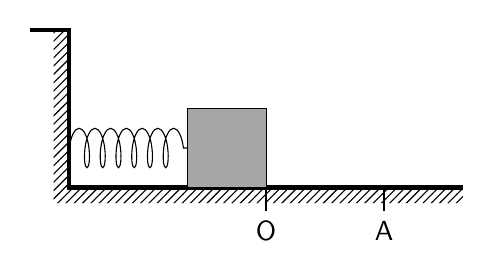
\begin{tikzpicture}
      \fill [pattern=north east lines] (5,0)--(0,0)--(0,2)--(-0.2,2)
      --(-0.2,-0.2)--(5,-0.2)--cycle;
      \draw[ultra thick] (5,0)--(0,0)--(0,2)--(-0.5,2);
      \draw[decoration={aspect=0.3,segment length=2mm, amplitude=2.5mm, coil},
        decorate] (0,0.5)--(1.5,0.5);
      \draw[fill=gray!70](1.5,0) rectangle(2.5,1);
      \draw[thick](2.5,0)--(2.5,-0.3) node[pos=1,below]{O};
      \draw[thick](4,0)--(4,-0.3) node[pos=1,below]{A};
    \end{tikzpicture}
  \end{center} 
  \begin{enumerate}[noitemsep]  
  \item In terms of the given quantities, at what distance from the equilibrium
    position is the potential energy of the mass equal to its kinetic energy?
  \item In terms of the given quantities, what is the acceleration of the mass
    when it is at the amplitude $A$?
  \end{enumerate}
%  \vspace{3in}
  \newpage
  
\item A mass oscillates in simple harmonic motion as shown by the position $x$
  vs. time $t$ graph below.
  \begin{center}
    \pic{.45}{oscillate.png}
  \end{center}
  \begin{enumerate}[noitemsep]  
  \item What is the frequency of oscillation?
  \item Write the equation that represents the speed of the mass as a function
    of time.
  \end{enumerate}
\end{enumerate}
\end{document}
